\label{chap:impl}

 \subsection{Hardware Details}

The hardware components used are the following:
\begin{itemize}

\item a SparrowDongle with two microcontrollers: The 8-bit ATMega128RFA1 which has an on-chip 2.4GHz wireless transceiver and the ATMega32U4, both from Atmel.

\item a SparrowV3.2  with an ATMega128RFA1 microcontroller 

\item a AR Parrot Drone v2.0

\item an laptop or mobile phone with android/ios for controlling the drone

\end{itemize}

Because of the addition of SparrowDongle, the drone's poliester hull has been carved a little in order to accomodate it.


\begin{figure}[ht] \centering
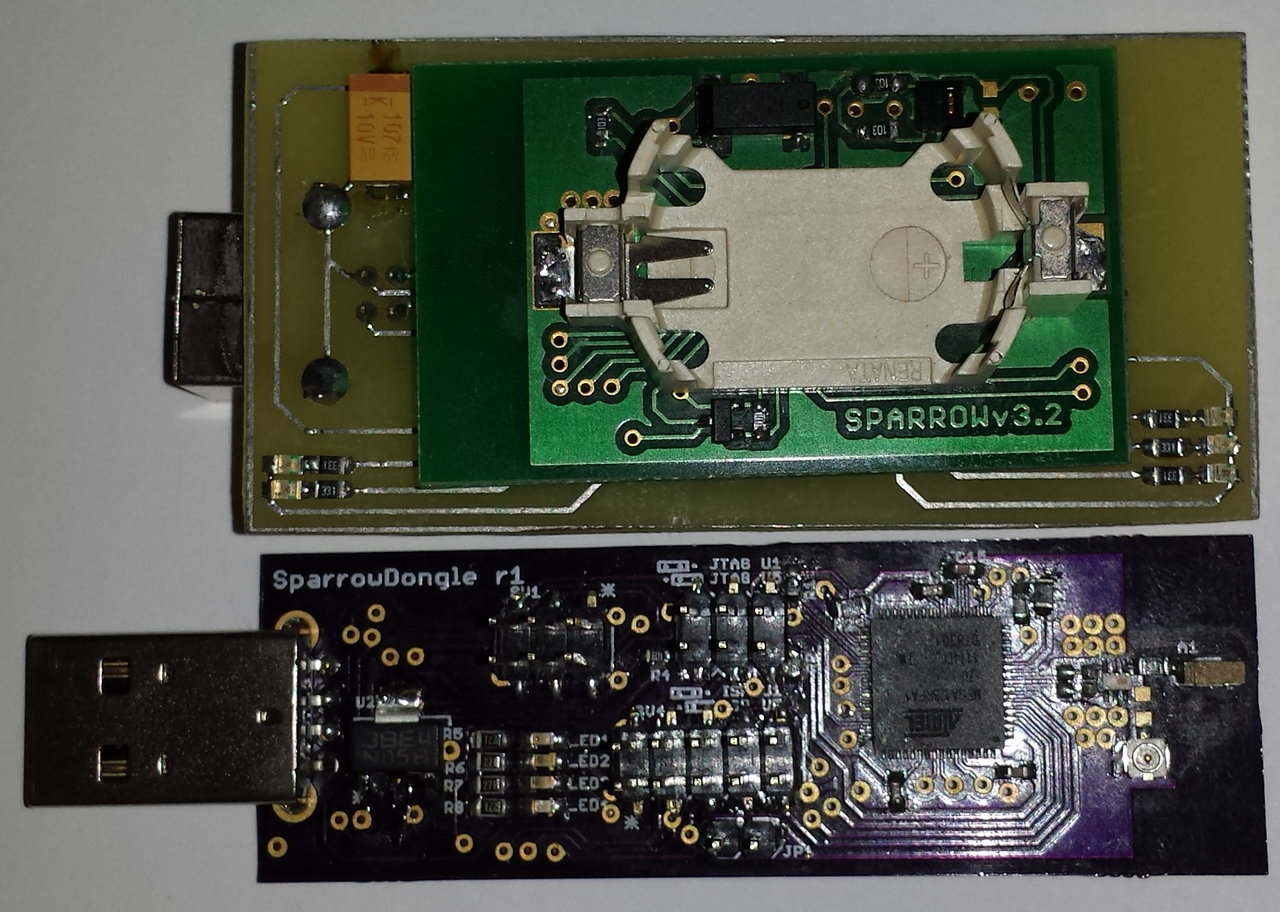
\includegraphics[width=0.5\textwidth]{img/sparrow.jpg} \caption{SparrowV3.2 and SparrowDongle} \end{figure}



\subsection{Software Implementation}

The SparrowDongle gateway dumps every data received on the serial. It is always in a listen for data state. When it receives the data, it sends back an ack to let the SparrowV3.2 know that it can begin sending the entire data to the mobile gateway.

The SparrowV3.2 node is sending periodicaly a small data packet to check if a gateway is available. When it receives the ack for the packet it starts sending the stored data to the gateway. The data sent can vary, from sensor readings, to debuging informations in order to check the state of the Wireless Sensor Network.

The data gattered by the gateway is saved into the AR Parrot Drone's internal memory. The data can be accesed at any time by any device connected to the drone's wireless network via ftp.
